\documentclass[12pt,letterpaper]{article}
\usepackage{graphicx,textcomp}
\usepackage{natbib}
\usepackage{setspace}
\usepackage{fullpage}
\usepackage{color}
\usepackage[reqno]{amsmath}
\usepackage{amsthm}
\usepackage{fancyvrb}
\usepackage{amssymb,enumerate}
\usepackage[all]{xy}
\usepackage{endnotes}
\usepackage{lscape}
\newtheorem{com}{Comment}
\usepackage{float}
\usepackage{hyperref}
\newtheorem{lem} {Lemma}
\newtheorem{prop}{Proposition}
\newtheorem{thm}{Theorem}
\newtheorem{defn}{Definition}
\newtheorem{cor}{Corollary}
\newtheorem{obs}{Observation}
\usepackage[compact]{titlesec}
\usepackage{dcolumn}
\usepackage{tikz}
\usetikzlibrary{arrows}
\usepackage{multirow}
\usepackage{xcolor}
\newcolumntype{.}{D{.}{.}{-1}}
\newcolumntype{d}[1]{D{.}{.}{#1}}
\definecolor{light-gray}{gray}{0.65}
\usepackage{url}
\usepackage{listings}
\usepackage{color}

\definecolor{codegreen}{rgb}{0,0.6,0}
\definecolor{codegray}{rgb}{0.5,0.5,0.5}
\definecolor{codepurple}{rgb}{0.58,0,0.82}
\definecolor{backcolour}{rgb}{0.95,0.95,0.92}

\lstdefinestyle{mystyle}{
	backgroundcolor=\color{backcolour},   
	commentstyle=\color{codegreen},
	keywordstyle=\color{magenta},
	numberstyle=\tiny\color{codegray},
	stringstyle=\color{codepurple},
	basicstyle=\footnotesize,
	breakatwhitespace=false,         
	breaklines=true,                 
	captionpos=b,                    
	keepspaces=true,                 
	numbers=left,                    
	numbersep=5pt,                  
	showspaces=false,                
	showstringspaces=false,
	showtabs=false,                  
	tabsize=2
}
\lstset{style=mystyle}
\newcommand{\Sref}[1]{Section~\ref{#1}}
\newtheorem{hyp}{Hypothesis}

\title{Problem Set 2}
\date{Sein Kim}
\author{Applied Stats/Quant Methods 1}

\begin{document}
	\maketitle
	
	\section*{Question 1: Political Science}
	
	The following table was created using the data from a study run in a major Latin American city.\footnote{Fried, Lagunes, and Venkataramani (2010). ``Corruption and Inequality at the Crossroad: A Multimethod Study of Bribery and Discrimination in Latin America. \textit{Latin American Research Review}. 45 (1): 76-97.} As part of the experimental treatment in the study, one employee of the research team was chosen to make illegal left turns across traffic to draw the attention of the police officers on shift. Two employee drivers were upper class, two were lower class drivers, and the identity of the driver was randomly assigned per encounter. The researchers were interested in whether officers were more or less likely to solicit a bribe from drivers depending on their class (officers use phrases like, ``We can solve this the easy way'' to draw a bribe). The table below shows the resulting data.
	
	\begin{table}[h!]
		\centering
		\begin{tabular}{l | c c c }
			& Not Stopped & Bribe requested & Stopped/given warning \\
			\hline
			Upper class & 14 & 6 & 7 \\
			Lower class & 7 & 7 & 1 \\
			\hline
		\end{tabular}
	\end{table}
	
	\begin{enumerate}
		\item[(a)] Calculate the $\chi^2$ test statistic by hand/manually (even better if you can do "by hand" in \texttt{R}).\\
		
		\noindent \textbf{Solution:}\\
		The $\chi^2$ statistic was computed as 
		\[
		\chi^2 = \sum \frac{(O - E)^2}{E}
		\]
		using expected frequencies from the row and column totals.
		
		\lstinputlisting[language=R, firstline=30, lastline=41]{PS02_SK.R}
		
		The result is $\chi^2 = 5.02$ with $df = 2$, which indicates a moderate difference from what would be expected under independence.
		
		\vspace{0.4cm}
		
		\item[(b)] Now calculate the p-value from the test statistic you just created (in \texttt{R}).\footnote{Remember frequency should be $>$ 5 for all cells, but let's calculate the p-value here anyway.}  What do you conclude if $\alpha = 0.1$?\\
		
		\noindent \textbf{Solution:}\\
		\lstinputlisting[language=R, firstline=42, lastline=44]{PS02_SK.R}
		
		The p-value is $p = 0.081$.  
		At $\alpha = 0.10$, since $p < 0.10$, we reject the null hypothesis and conclude that there is some evidence of an association between driver class and police response.
		
		\vspace{0.5cm}
		
		\item[(c)] Calculate the standardized residuals for each cell and put them in the table below.\\
		
		\noindent \textbf{Solution:}\\
		\lstinputlisting[language=R, firstline=46, lastline=53]{PS02_SK.R}
		
		\begin{table}[H]\centering
			\caption{\footnotesize Standardized residuals from chi-square test.}
			\begin{tabular}{l|ccc}
				& Not Stopped & Bribe Requested & Warning Given \\
				\hline
				Upper class & 0.33 & \textbf{-1.64} & 1.52 \\
				Lower class & -0.33 & \textbf{+1.64} & -1.52 \\
			\end{tabular}
		\end{table}
		
		\noindent Residuals exceeding $\pm 2$ indicate unusually large deviations.
		
		\vspace{0.2cm}
		The “Lower–Bribe Requested” cell shows a positive residual (+1.64). Lower-class drivers were asked for bribes more frequently than expected, suggesting that police officers may have shown some bias against lower-class drivers. In contrast, upper-class drivers were relatively less likely to be asked for bribes, consistent with unequal enforcement patterns.
		
		\vspace{0.4cm}
		
		\item[(d)] How might the standardized residuals help you interpret the results?\\
		Large positive residuals indicate overrepresentation of observations relative to independence, and large negative residuals indicate underrepresentation.  
		Here, the pattern suggests unequal treatment by class: lower-class drivers were more likely to face bribery requests.
	\end{enumerate}
	
	\newpage
	\section*{Question 2: Economics}
	
	Chattopadhyay and Duflo were interested in whether women promote different policies than men.\footnote{Chattopadhyay and Duflo. (2004). ``Women as Policy Makers: Evidence from a Randomized Policy Experiment in India. \textit{Econometrica}. 72 (5), 1409-1443.} 
	Answering this question with observational data is difficult due to confounding variables. Hence, they exploit a randomized policy experiment in India, where since the mid-1990s, one-third of village council head positions have been randomly reserved for women. 
	A subset of the data from West Bengal is available at \url{https://raw.githubusercontent.com/kosukeimai/qss/master/PREDICTION/women.csv}.
	
	\begin{enumerate}
		\item[(a)] State a null and alternative (two-tailed) hypothesis.\\
		
		\noindent \textbf{Solution:}
		\[
		H_0: \beta_{\text{reserved}} = 0 \quad \text{vs.} \quad H_1: \beta_{\text{reserved}} \neq 0
		\]
		
		\vspace{0.3cm}
		
		\item[(b)] Run a bivariate regression to test this hypothesis in \texttt{R} (include your code!).\\
		
		\noindent \textbf{R Code:}
		\lstinputlisting[language=R, firstline=62, lastline=74]{PS02_SK.R}
		
		\noindent \textbf{Result:}\\
		The estimated coefficient is $\hat{\beta}_1 = 9.15$ \; ($SE = 3.72$, $t = 2.46$, $p = 0.016$).
		
		\vspace{0.3cm}
		\item[(c)] Interpret the coefficient estimate for reservation policy.\\
		
		\noindent Since $p < 0.05$, the coefficient on the reservation dummy, $\hat{\beta}_1 = 9.15$ \; ($SE = 3.72$), indicates that, on average, villages reserved for women had approximately nine additional water facilities compared to non-reserved ones. This effect is statistically significant ($p = 0.016$) and suggests that female leadership increases investment in public goods such as water facilities.
		
		\begin{figure}[H]\centering
			\caption{\footnotesize Number of new/repaired water facilities by reservation status. Red dots represent group means; the distribution clearly shows higher central tendency for reserved villages, consistent with the positive estimated coefficient.}
			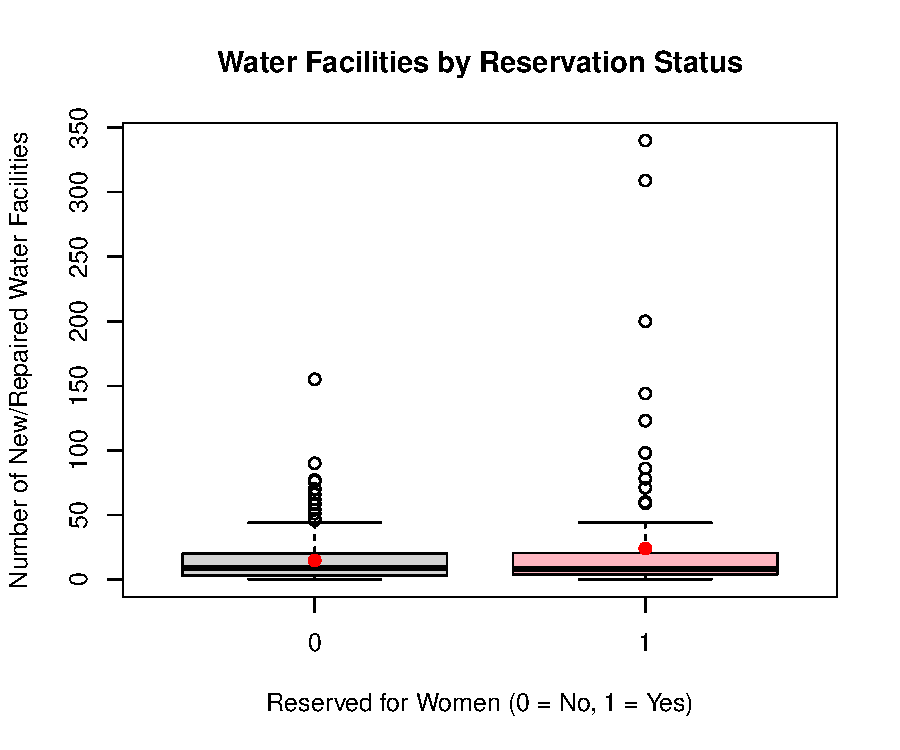
\includegraphics[width=0.65\textwidth]{q2_water_by_reserved.pdf}
		\end{figure}
		
	\end{enumerate}
	
\end{document}